\section{Platform Effects and Sector Values}
\label{section:params}

\subsection{Data Quantization}

In order to explore the sensitivity of the online sector analysis technique with respect to
data quantization effects, we simulated the possible degradation of the sector bound
measurement as the data precision increased.  All Simulink simulation runs in these
experiments were sampled 
at 50 Hz.  The model under test adds an input filter to remove frequencies right near
the Nyquist frequency (to avoid the difficulties encountered earlier).  We simulated
the fixed-point quantization effects by adding an appropriate noise component to the
system inputs (zero-mean Gaussian noise with variance $\frac{2^{-2bits}}{12}$. 
For the chosen input signal 100 seconds was sufficient to get
the sector measurement to settle.  A more rigorous investigation is certainly needed, 
but our initial goal was to obtain a rough idea of the sensitivity of the sector to 
quantization without deploying and debugging all of the different configurations.  

\begin{table}[htb]
\centering
\begin{tabular}[width=\columnwidth]{ | l | l | l | l | l | }
\hline
\textbf{Quant Level} & \textbf{Ang Velocity} & \textbf{Angle} & \textbf{Velocity} & \textbf{Position} \\
\hline \hline
Gain bound  & -4.0000 & -1.0951 & -1.0000 & -18.0505 \\
$a > -\frac{1}{k}$ & & & & \\
\hline \hline
double & -3.0116 & -0.9237 & -0.7252 & -1.0625 \\
\hline
single & -3.0127 & -0.9237 & -0.7267 & -1.0625 \\
\hline
fix16 & -3.0127 & -2.1673 & -0.7266 & -12.0967 \\
\hline
fix14 & -3.0126 & -2.1834 & -0.7258 & -26.7733 \\
\hline
fix10 & -7.5519 & -2.1845 & -0.5887 & -29.1194 \\
\hline \hline
Gain bound & -4.0000 & -1.0951 & -1.0000 & -18.0505 \\
\hline
\end{tabular}
\caption{ Sector value under different quantization levels.}
\label{tab:quant}
\end{table}

\begin{figure}[htb]
\centering
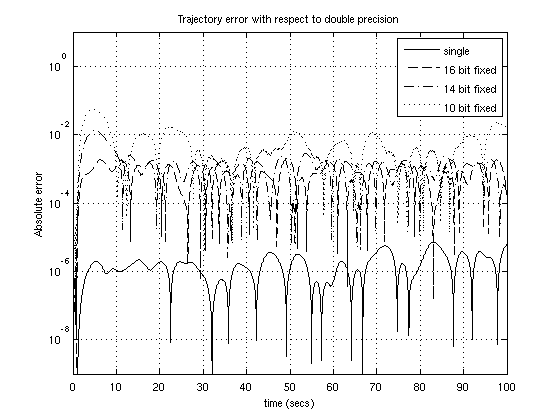
\includegraphics[width=\columnwidth]{figures/quantization_error}
    \caption{Output tracking error over time with respect to data quantization differences. The reference input is a square wave.}
    \label{fig:quant_err}
\end{figure}

Table \ref{tab:quant} presents sector values for the various simulated
quantization levels.  Different control loops degrade at different points under the 
current input.  The idea was to choose an input with a wide range of frequency content,
and overdrive the system slightly.  Our design did not perform well with fixed-point
quantization, suggesting that an operational loss of data precision could present a
risk of destabilizing our control system.  For comparison, Fig. \ref{fig:quant_err} 
displays the relative tracking error for each of the quantization levels.  The sector
bounds did not vary quite as smoothly with respect to quantization as did the position 
output.  It appears that the sector analyzer is sufficiently sensitive to explore these
effects.

\subsection{Scheduling and Delay Effects}

To further explore the sensitivity of the design and to validate the search technique,
we simulated a wide range of synchronous (integer) delay values for the links between the 
components.  This captures effects both of actual network delay as well as delays 
introduced by our calculated static schedule \cite{sched:analysis}.
We collected data over the input and parameter ranges specified in Table \ref{tab:testparams} 
Even our relatively small and simple design required 472,392 data sets to assess the 
behavior of the sector bounds with respect to the input and parameter design spaces.
We opted for an exhaustive simulation set, as the required compute power and storage space were
available.  Still, the simulations took approximately three days to run.
Each simulation was driven by a square wave input with the specified amplitude and 
frequency.  Note that the input amplitudes correspond to slightly unrealistic input levels, as
overdriving the control system seemed to help explore the full range of the sector values.

\begin{table}[htb]
\centering
\begin{tabular}[width=\columnwidth]{ | l | l | }
\hline
\textbf{Quantity} & \textbf{Simulation Values} \\
\hline
Delay from Plant & 0--8 (ticks)  \\
 to Data Handler $D_{PH}$ & \\
\hline
Delay from Data Handler & 0--8 (ticks)  \\
 to Outer Loop $D_{HO}$ & \\
\hline
Delay from Outer Loop & 0--8 (ticks)  \\
 to Inner Loop $D_{OI}$ & \\
\hline
Delay from Inner Loop & 0--8 (ticks)  \\
  to Plant $D_{IP}$ & \\
\hline
Reference input & .20, .10, .033 (Hz) \\
frequency & \\
\hline
Sample rate & 25, 35, 50, 75,  \\
 & 90, 100 (Hz) \\
\hline
Reference input & 0.5, 1, 2, 4 (m)  \\
 amplitude & \\
\hline
\end{tabular}
\caption{ Parameter test ranges. }
\label{tab:testparams}
\end{table}

Surprisingly, no immediate pattern emerged from the data analysis. Our hope was that the
change in total delay ($D_T = D_{PH} + D_{HO} + D_{OI} + D_{IP}$) through the system would 
correlate well with changes in the sector values measured for any given set point of the 
other parameters.  Slicing the data separately by sample rate, by amplitude, and by 
frequency showed roughly the same range of sector values for all runs.  Interestingly, the 
total delay also did not seem to change the pattern. 

Our preliminary observation is that (in general) system behavior with respect to the sector
bounds depends more on the distribution of delays through the system than on any other 
parameter.  Unfortunately, our early investigation into the delay parameter dependence 
shows some unusual patterns.   Fig. \ref{fig:delaydata} illustrates
this concept for a single set point (Input Freq = .033 Hz, Amplitude = 0.5, and Sample rate
= 100 Hz).  Searching for delay patterns in the generated data, the outlying points around 
$a = -0.9$ roughly correspond to the condition
$D_{PH} > 0 \wedge D_{HO} = 0 \wedge D_{OI} = 0 \wedge D_{IP} > 0$, 
where the delay is split between the links before the controller and after the controller
(between the inner loop and the plant). The ordering and scheduling of the data flow and execution
for the inner and outer loops in this case are fully sequential, as they incur no sample ticks
between their invocations and transfers. A more careful investigation is necessary in order to be 
able to characterize the space of possible delay values and discern meaningful patterns.

\begin{figure}[htb]
\centering
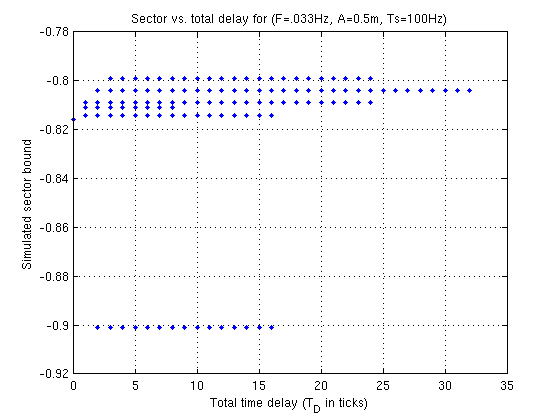
\includegraphics[width=\columnwidth]{figures/sectvstotaldelay}
    \caption{The sector variations seem to depend more on the distribution of delays in the 
individual links rather than on the delay values themselves.}
    \label{fig:delaydata}
\end{figure}

Our conclusion from this preliminary investigation is that our controller is reasonably
insensitive to delays, and therefore the sector analysis might not detect delay anomalies in
the system, depending on where in the communication chain they occur.  Repeating the analysis
with a known delay-sensitive control structure would provide a good comparison, as well as trying
a wider range of parameter and input conditions.
